\documentclass[10pt]{beamer}

\usepackage{mathtools}
\usepackage{bm}
\usetheme{CambridgeUS}
\usecolortheme{dolphin}

\usepackage{graphicx}
\graphicspath{ {./images/} }

\usepackage{tabularx}
\usepackage{caption}
\usepackage{subcaption}
\usepackage{float}

\usepackage{biblatex}
\addbibresource{references.bib}

% set colors
\definecolor{myNewColorA}{RGB}{115, 0, 10} % garnet
\setbeamercolor*{palette primary}{bg=myNewColorA, fg=white}
\setbeamercolor*{palette secondary}{bg=myNewColorA, fg=white}
\setbeamercolor*{palette tertiary}{bg=myNewColorA, fg=white}
\setbeamercolor*{titlelike}{fg=myNewColorA}
\setbeamercolor*{title}{bg=myNewColorA, fg = white}
\setbeamercolor*{item}{fg=myNewColorA}
\setbeamercolor*{caption name}{fg=myNewColorA}
\usefonttheme{professionalfonts}

\titlegraphic{
\includegraphics[height=1.5cm]{images/uofsc logo.jpg}}

\setbeamerfont{title}{size=\large}
\setbeamerfont{subtitle}{size=\small}
\setbeamerfont{author}{size=\small}
\setbeamerfont{date}{size=\small}
\setbeamerfont{institute}{size=\small}

\title[Dimensionality Reduction in the Parameter Space]{Dimensionality Reduction in the Parameter Space}
\subtitle{Active Subspace and Nonlinear Level Set Learning Techniques}
\author[Malcolm Gaynor and Cade Stanley]{Malcolm Gaynor and Cade Stanley \\{\scriptsize Advisor: Zhu Wang} \\{\scriptsize Graduate Student: Yuwei Geng}}

\institute[]{U of SC Summer REU: Summer School on Mathematical Foundation of Data Science}
\date[July 15, 2022]{July 15, 2022}

%------------------------------------------------------------
%This block of commands puts the table of contents at the 
%beginning of each section and highlights the current section:
%\AtBeginSection[]
%{
%  \begin{frame}
%    \frametitle{Contents}
%    \tableofcontents[currentsection]
%  \end{frame}
%}

\AtBeginSection[]{
  \begin{frame}
  \vfill
  \centering
  \begin{beamercolorbox}[sep=8pt,center,shadow=true,rounded=true]{title}
    \usebeamerfont{title}\insertsectionhead\par%
  \end{beamercolorbox}
  \vfill
  \end{frame}
}
%------------------------------------------------------------

\begin{document}
\frame{\titlepage}

%\begin{frame}
%\frametitle{Contents}
%\tableofcontents
%\end{frame}
%------------------------------------------------------------
%\section{Introduction}
\begin{frame}{Introduction: The Curse of Dimensionality}
\begin{itemize}
    \item \textbf{Problem}: when the number of parameters increases, the costs of computing the function increase exponentially 
    
    \item \textbf{Goal}: reduce costs of performing parameter studies for complex, high-dimensional functions
    
    \item \textbf{Idea}: find important directions in the parameter space
    \begin{itemize}
        \item directions along which most of the function's variability can be observed
    \end{itemize}
\end{itemize}

\begin{figure}[H]
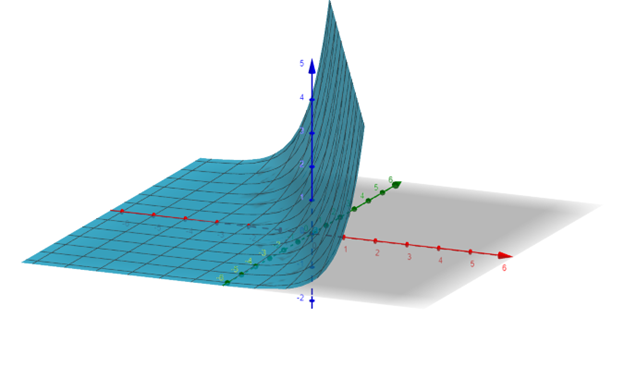
\includegraphics[width=2in]{images/exp example (3d).png}
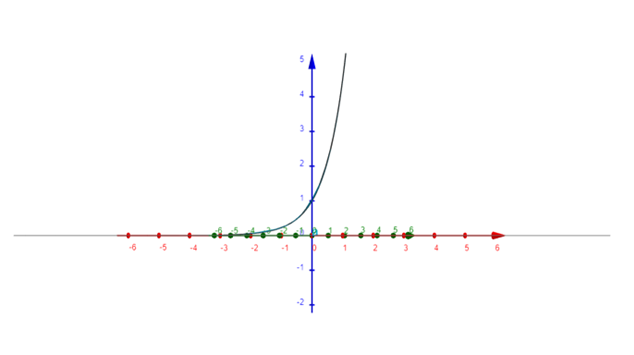
\includegraphics[width=2in]{images/exp example (2d).png}
\caption{A 2D exponential function that collapses into 1 dimension when rotated.}
\end{figure}
\end{frame}

\begin{frame}{Two Approaches}
\begin{itemize}\itemsep20pt
    \item \textbf{Active Subspace (AS) Method:} a linear approach to finding important directions, based on eigendecomposition of the gradient covariance matrix
    \item \textbf{Nonlinear Level Set Learning (NLL) Method:} a nonlinear approach to parameterizing level sets in a lower dimension, based on reversible neural networks called RevNets 
\end{itemize}
\end{frame}

\section{The Active Subspace Method}
\begin{frame}{Finding the Active Subspace}
\begin{itemize}
    \item Suppose $f$ is a $d$-dimensional function with domain $\Omega \subset \mathbb{R}^d$

    \item \textbf{Goal:} find a subspace of $\Omega$ where changes in the parameters explain most of $f$'s variability
    
    \item \textbf{Gradient Covariance Matrix:} $\bm{C} = \mathbb{E}\left[\left(\nabla_{\bm{x}}f\right)\left(\nabla_{\bm{x}}f\right)^\top \right]$
\end{itemize}
\textbf{Procedure:}
\begin{itemize}
    \item Approximate $\bm{C}$ using $\hat{\bm{C}}=\frac{1}{M}\sum_{i=1}^{M}(\nabla_{\bm{x}} f_i)(\nabla_{\bm{x}} f_i)^\top$
    %\begin{itemize}
    %    \item $\nabla_{\bm{x}} f_i = \nabla_{\bm{x}} f(x_i)$, where $x_i$ is randomly sampled from the function's domain by taking $M$ random samples
    %\end{itemize}
    
    \item Perform eigendecomposition: $\hat{\bm{C}} = \bm{W}\boldsymbol{\Lambda}\bm{W}^\top$
    
    \item Search for a large gap between eigenvalues, and partition at the gap:
    \begin{align*}
        \bm{W} = 
        \begin{bmatrix}
            \bm{W}_1 & \bm{W}_2
        \end{bmatrix}
        && \bm{\Lambda} =
        \begin{bmatrix}
            \bm{\Lambda}_1 & \\
            & \bm{\Lambda}_2
        \end{bmatrix}
    \end{align*}
    
    \item $\bm{W}_1$ holds the eigenvectors that make up the active subspace, $\bm{\eta}_1, \dots, \bm{\eta}_n$
    
    \item $\bm{\Lambda}_1$ holds the eigenvalues corresponding to those eigenvectors, $\lambda_1, \dots, \lambda_n$
\end{itemize}
\end{frame}

\begin{frame}{Visualizing the Active Subspace}
\begin{itemize}\itemsep20pt
    \item \textbf{Eigenvalue plot:} plot all eigenvalues in decreasing order - visualize the gaps
    
    \item \textbf{Sufficient summary plot:} plot the function value against the linear combinations $\bm{\eta}_1^\top \bm{x}, \dots, \bm{\eta}_n^\top \bm{x}$
    
    \item \textbf{Sensitivity chart:} compare the function's sensitivity to its original parameters with its sensitivity to the new active and inactive dimensions 
    
    \item \textbf{Activity score:} analyze the activity of the parameters in the eigenvectors making up the active subspace
    
    \item \textbf{Grid transformation:} apply the active subspace transformation to the original parameter space and visualize the transformed space
\end{itemize}
\end{frame}

\begin{frame}{A Simple Example}
\begin{center}
    $f(\bm{x})=\frac{1}{2}\sin(2\pi(x_1+x_2))+1$
\end{center}
\begin{figure}
\begin{subfigure}{0.3\textwidth}
    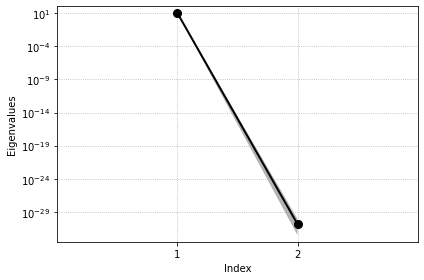
\includegraphics[width=1.25in]{images/f1 eigen.png}
    \caption{Eigenvalue plot}
\end{subfigure}
\begin{subfigure}{0.3\textwidth}
    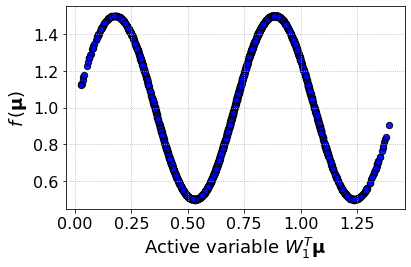
\includegraphics[width=1.25in]{images/f1 AS.png}
    \caption{Sufficient summary plot}
\end{subfigure}
\begin{subfigure}{0.3\textwidth}
    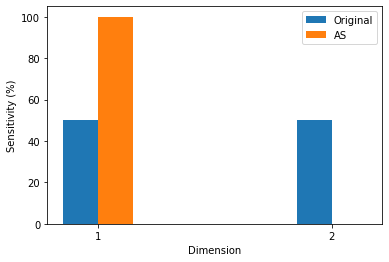
\includegraphics[width=1.25in]{images/f1sens.png}
    \caption{Sensitivity chart}
\end{subfigure}
\begin{subfigure}{0.3\textwidth}
    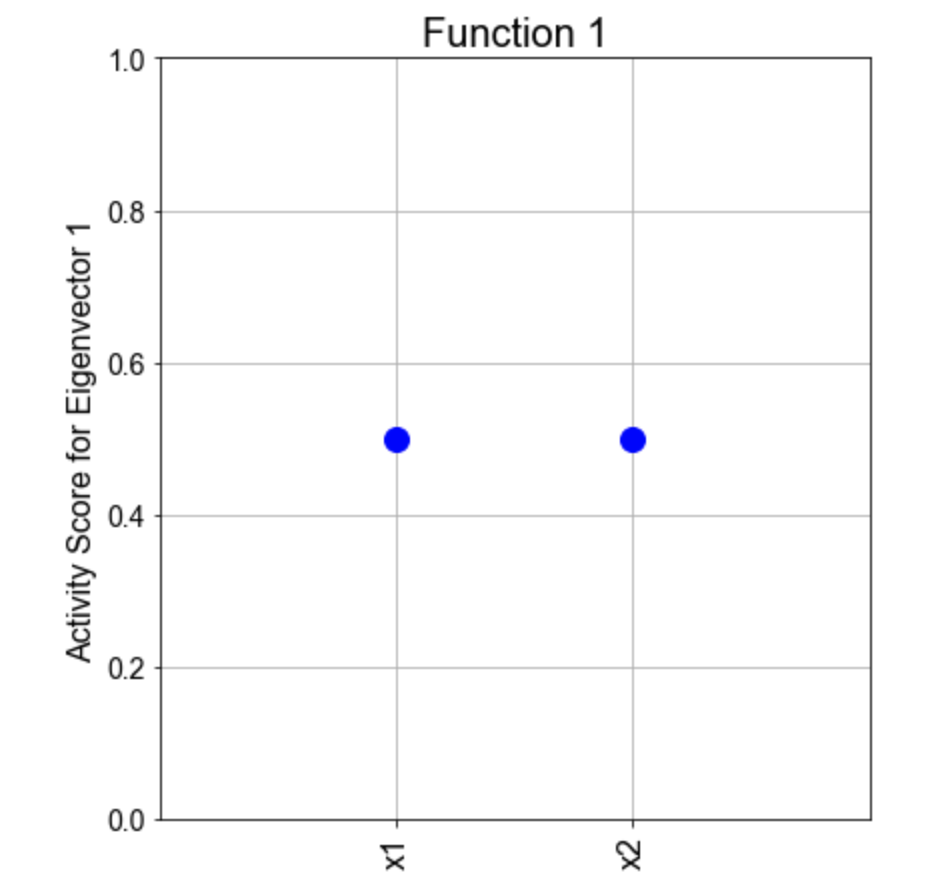
\includegraphics[height=1in,width=1.25in]{images/f1ES.png}
    \caption{Activity score}
\end{subfigure}
\begin{subfigure}{0.3\textwidth}
    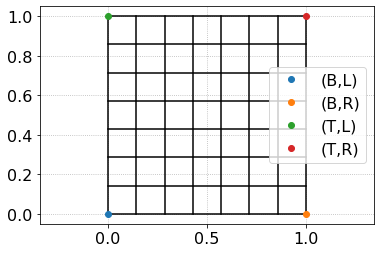
\includegraphics[width=1.25in]{images/f1 grid.png}
    \caption{Original parameter space}
\end{subfigure}
\begin{subfigure}{0.3\textwidth}
    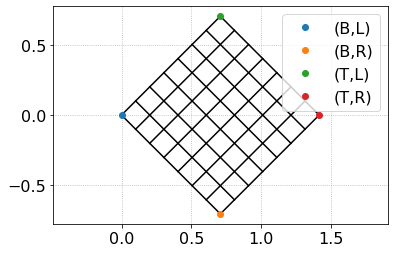
\includegraphics[width=1.25in]{images/f1 AS mesh.png}
    \caption{Transformed parameter space}
\end{subfigure}
\end{figure}
\end{frame}


\section{The Nonlinear Level Set Learning Method}
\begin{frame}{Development}
\begin{itemize}\itemsep20pt
    \item Suppose $f$ is a $d$-dimensional function with domain $\Omega \subset \mathbb{R}^d$
    
    \item \textbf{Goal:} create a bijective nonlinear transformation $\bm{g}: \Omega \rightarrow \mathbb{R}^d$, where for any $\bm{x} \in \Omega$, $\bm{g}(\bm{x}) = \bm{z}$ so that $\bm{z}$ has a small number of ``active'' inputs
    
    \item We want to write $\bm{z} = (\bm{z}_1, \bm{z}_2)$ so that $f \circ \bm{g}^{-1}$ is sensitive only to changes in $\bm{z}_1$, where $\bm{z}_1$'s dimension is much smaller than $d$.  
    
    \item $f \circ \bm{g}^{-1}(\bm{z}) = f(\bm{x})$, so approximating $f \circ \bm{g}^{-1}$ using only the active components in $\bm{z}_1$ will let us approximate $f$ in lower dimensions
\end{itemize}
\end{frame}

\begin{frame}{The Neural Network}
    \begin{itemize}
        \item The transformation $\bm{g}$ is trained using a RevNet with the following structure:
        $$
        \begin{cases}
            \bm{u}_{n+1} = \bm{u}_n + h\bm{K}_{n,1}^\top\boldsymbol{\sigma}(\bm{K}_{n,1}\bm{v}_n + \bm{b}_{n,1}) \\
            \bm{v}_{n+1} = \bm{v}_n - h\bm{K}_{n,2}^\top \boldsymbol{\sigma}(\bm{K}_{n,2}\bm{u}_{n+1} + \bm{b}_{n,2}) 
        \end{cases},
        $$ for $n = 0, 1, \dots, N-1$.
        
        \begin{itemize}
            \item $h \in \mathbb{R}$ is the time step
        
            \item $\boldsymbol{\sigma}$ is the activation function (usually chosen as $tanh$)
        
            \item $\bm{K}_{n,1}, \bm{K}_{n,2}$ are weight matrices, and $\bm{b}_{n,1}, \bm{b}_{n,2}$ are bias vectors, which are all updated according to the loss function
        \end{itemize}
        
        \item Letting $\bm{x} =
                    \begin{bmatrix}
                    \bm{u}_0 \\
                    \bm{v}_0
                    \end{bmatrix}$ and
                    $\bm{z} = 
                    \begin{bmatrix}
                    \bm{u}_N \\
                    \bm{v}_N
                    \end{bmatrix}$,
        the network yields the transformation $\bm{g}(\bm{x}) = \bm{z}$
    \item When using the RevNet, it is also necessary to specify the number of layers, the active dimension, the learning rate, and the number of epochs, along with the time step and the activation function.  
    \end{itemize}   
\end{frame}


\begin{frame}{The Loss Function}
\begin{itemize}
    \item The Loss Function is used to train the RevNet with the structure outlined above
    \item There are two parts to the loss function, $L_1$ and $L_2$, both of which depend on the Jacobian matrix of the inverse transformation $\bm{g}^{-1}$
    \begin{itemize}
        \item Jacobian matrix: $$J(z)=[J_1(z),J_2(z),\dots J_d(z)] \mbox{ where each } J_i(z)=\left (\frac{\partial x_1}{\partial z_i}(z),\dots \frac{\partial x_d}{\partial z_i}(z) \right )^\top$$
        \item First component: $$L_1:=\sum_{s=1}^{M}\sum_{i=1}^{d}  \left[ \omega_i \left \langle \frac{J_i(z^{(s)})}{||J_i(z^{(s)})||_2}, \nabla f(x^{(s)})\right \rangle \right]^2,$$ where $\omega_1, \dots, \omega_d$ are weights (0 or 1) on each dimension.  
        \item Second component: $L_2:=(\mbox{det}(J)-1)^2$
    \end{itemize}
    \item \textbf{Final loss function:} $L:=L_1+\lambda L_2$, where $\lambda$ is a constant to be chosen by the user that balances the two terms 
\end{itemize}
\end{frame}

\begin{frame}{A Simple Example}
\begin{center}
    $f(\bm{x}) = x_1^3+x_2^3+0.2x_1+0.6x_2$
\end{center}
\begin{figure}
\begin{subfigure}{0.3\textwidth}
    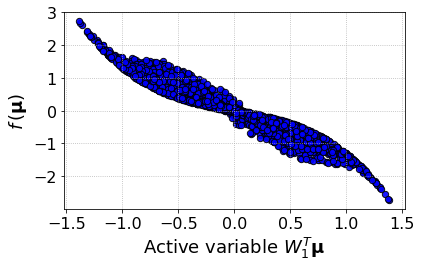
\includegraphics[width=1.25in]{images/f3 AS.png}
    \caption{AS plot}
\end{subfigure}
\begin{subfigure}{0.3\textwidth}
    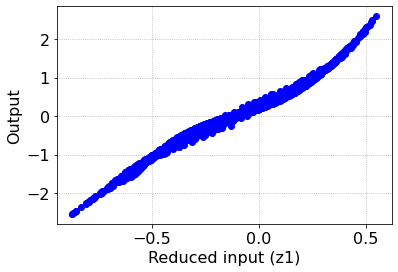
\includegraphics[width=1.25in]{images/f3nll.png}
    \caption{NLL plot}
\end{subfigure}
\begin{subfigure}{0.3\textwidth}
    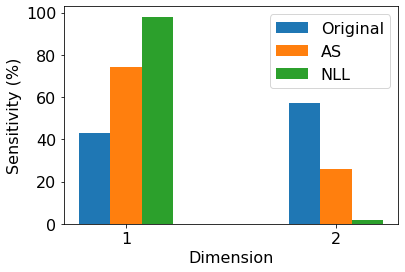
\includegraphics[width=1.25in]{images/f3 sens.png}
    \caption{Sensitivity chart}
\end{subfigure}
\begin{subfigure}{0.3\textwidth}
    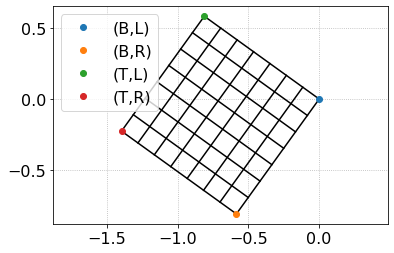
\includegraphics[width=1.125in]{images/f3 AS mesh.png}
    \caption{AS transformation}
\end{subfigure}
\begin{subfigure}{0.3\textwidth}
    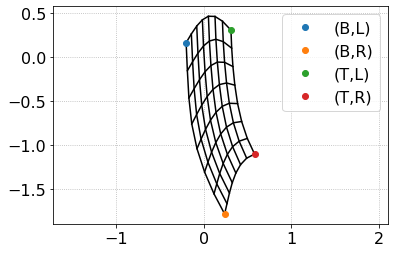
\includegraphics[width=1.25in]{images/f3nllmesh.png}
    \caption{NLL transformation}
\end{subfigure}
\end{figure}
\end{frame}


\section{Real-World Applications}
\begin{frame}{Wing Weight Function}

\begin{figure}
\begin{subfigure}{0.3\textwidth}
    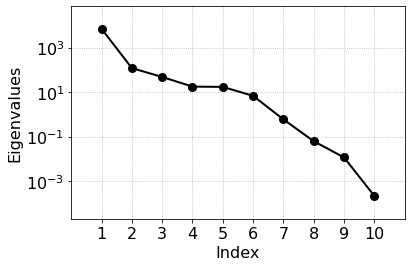
\includegraphics[height=1.25in,width=1.5in]{images/wingeigen.png}
    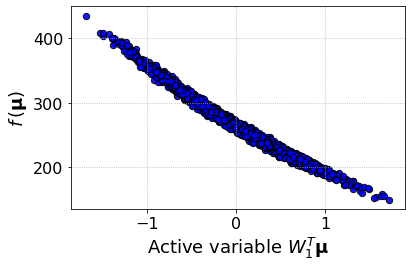
\includegraphics[height=1.25in,width=1.5in]{images/wingas.png}
    \caption{AS method}
\end{subfigure}
\hfill
\begin{subfigure}{0.3\textwidth}
    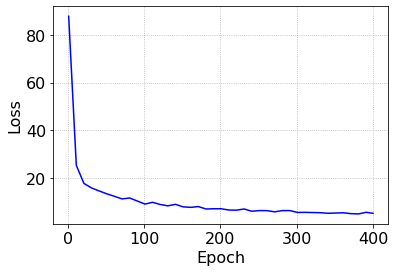
\includegraphics[height=1.25in,width=1.5in]{images/wingloss.png}
    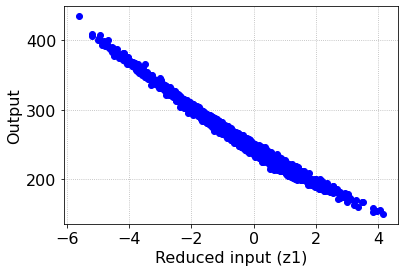
\includegraphics[height=1.25in,width=1.5in]{images/wingnll2.png}
    \caption{NLL method}
\end{subfigure}
\hfill
\begin{subfigure}{0.3\textwidth}
    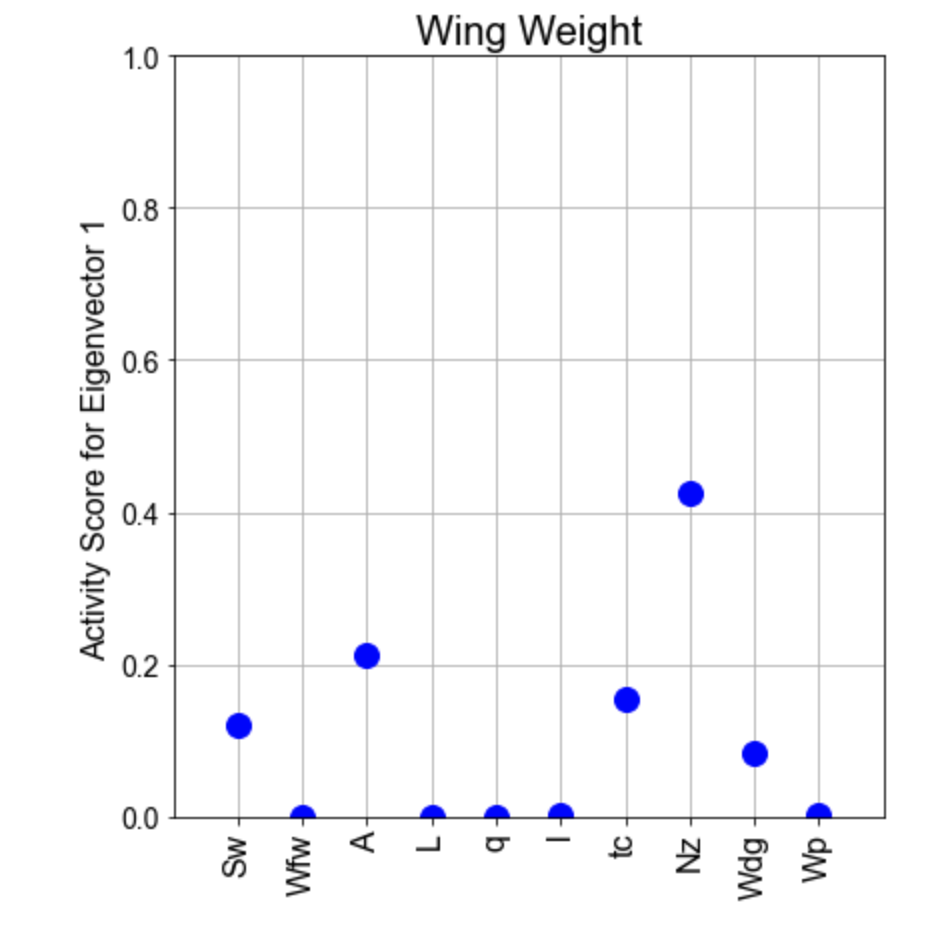
\includegraphics[height=1.25in,width=1.5in]{images/WingEC.png}
    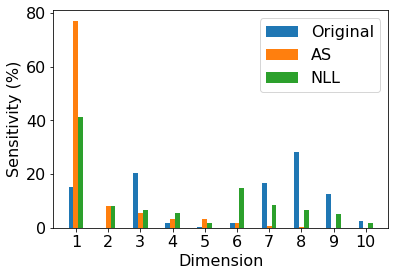
\includegraphics[height=1.25in,width=1.5in]{images/wingsens.png}
    \captionsetup{justification=centering}
    \caption{Activity score and sensitivity comparison}
\end{subfigure}
\end{figure}
\end{frame}


\begin{frame}{Piston Simulation Function}
\begin{figure}
\begin{subfigure}{0.3\textwidth}
    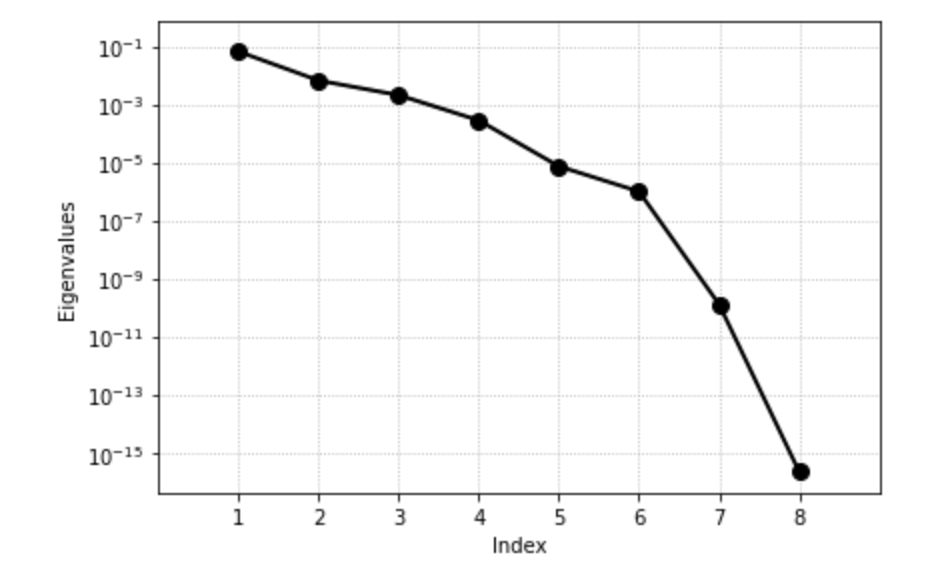
\includegraphics[height=1.25in,width=1.5in]{images/pistoneigen (1).png}
    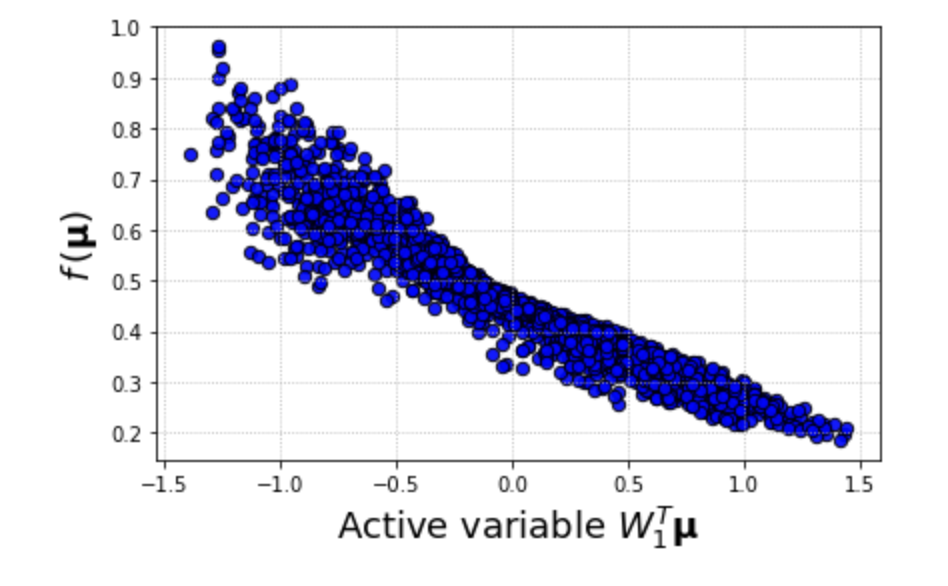
\includegraphics[height=1.25in,width=1.5in]{images/pistonas.png}
    \caption{AS method}
\end{subfigure}
\hfill
\begin{subfigure}{0.3\textwidth}
    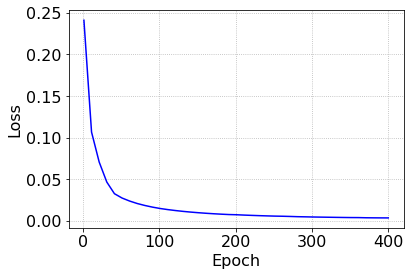
\includegraphics[height=1.25in,width=1.5in]{images/Pistonloss.png}
    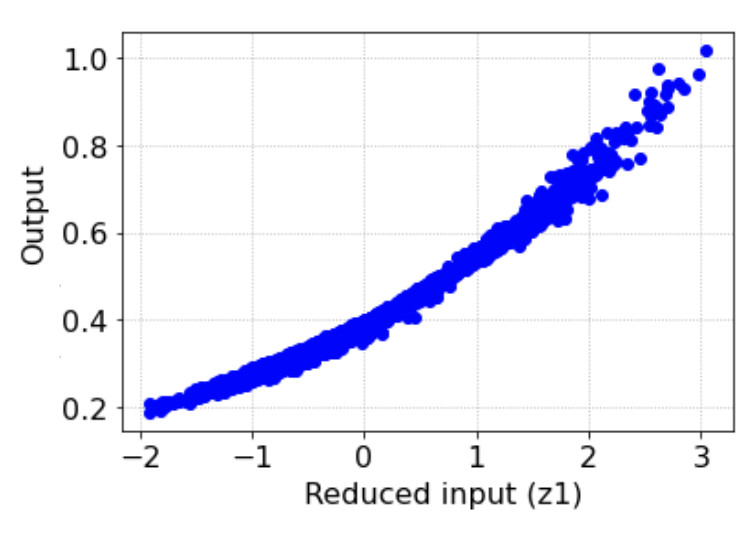
\includegraphics[height=1.25in,width=1.5in]{images/newPistonnll.png}
    \caption{NLL method}
\end{subfigure}
\hfill
\begin{subfigure}{0.3\textwidth}
    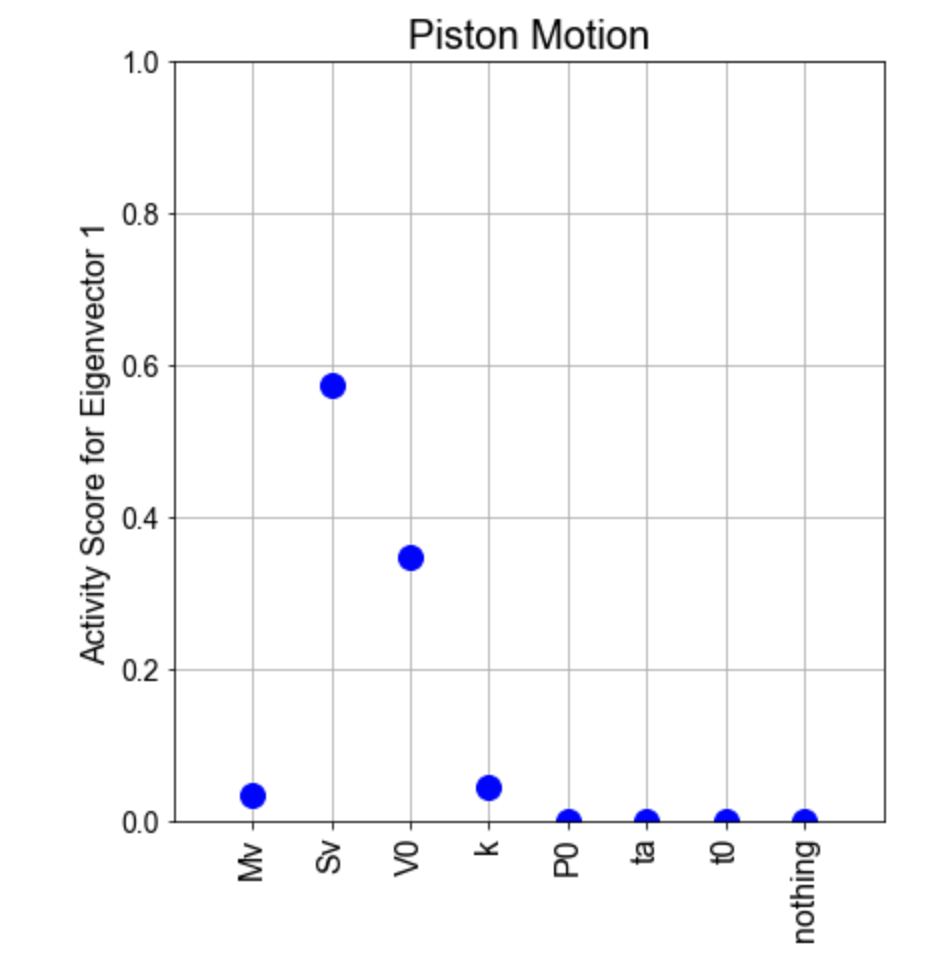
\includegraphics[height=1.25in,width=1.5in]{images/PEC.png}
    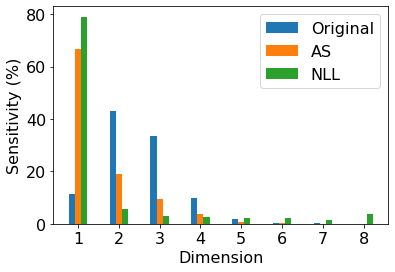
\includegraphics[height=1.25in,width=1.5in]{images/piston sens.png}
    \captionsetup{justification=centering}
    \caption{Activity score and sensitivity comparison}
\end{subfigure}
\end{figure}
\end{frame}


\begin{frame}{OTL Circuit Function}
\begin{figure}
\begin{subfigure}{0.3\textwidth}
    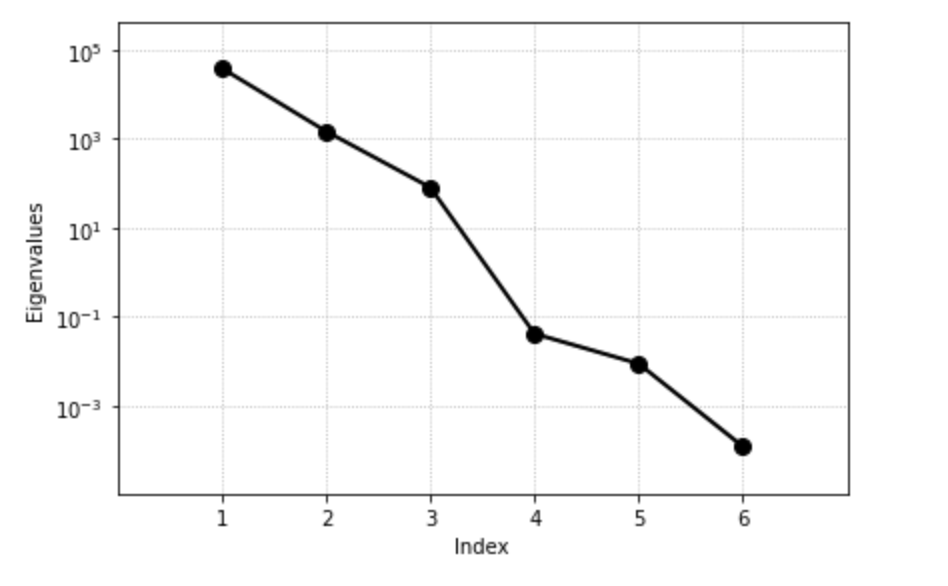
\includegraphics[height=1.25in,width=1.5in]{images/circuiteigen.png}
    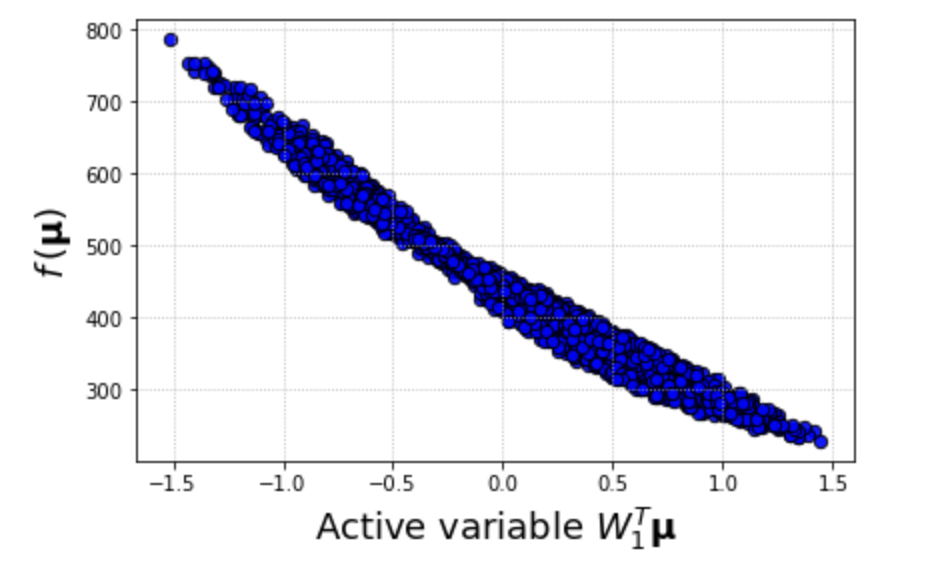
\includegraphics[height=1.25in,width=1.5in]{images/circuitas.png}
    \caption{AS method}
\end{subfigure}
\hfill
\begin{subfigure}{0.3\textwidth}
    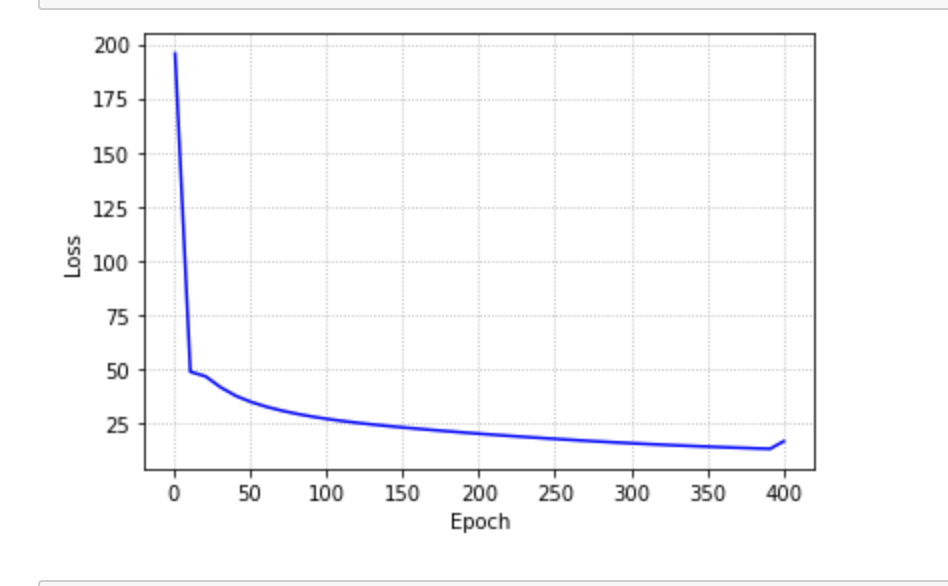
\includegraphics[height=1.25in,width=1.5in]{images/circuitloss.png}
    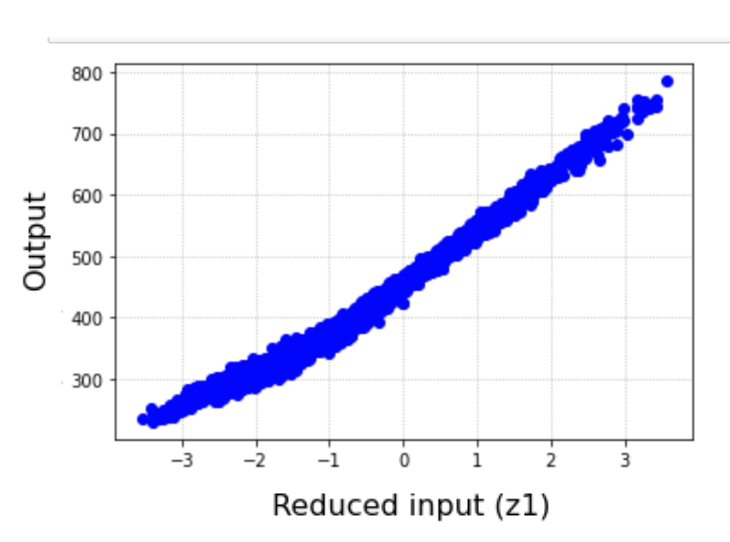
\includegraphics[height=1.25in,width=1.5in]{images/newcircuitnll.png}
    \caption{NLL method}
\end{subfigure}
\hfill
\begin{subfigure}{0.3\textwidth}
    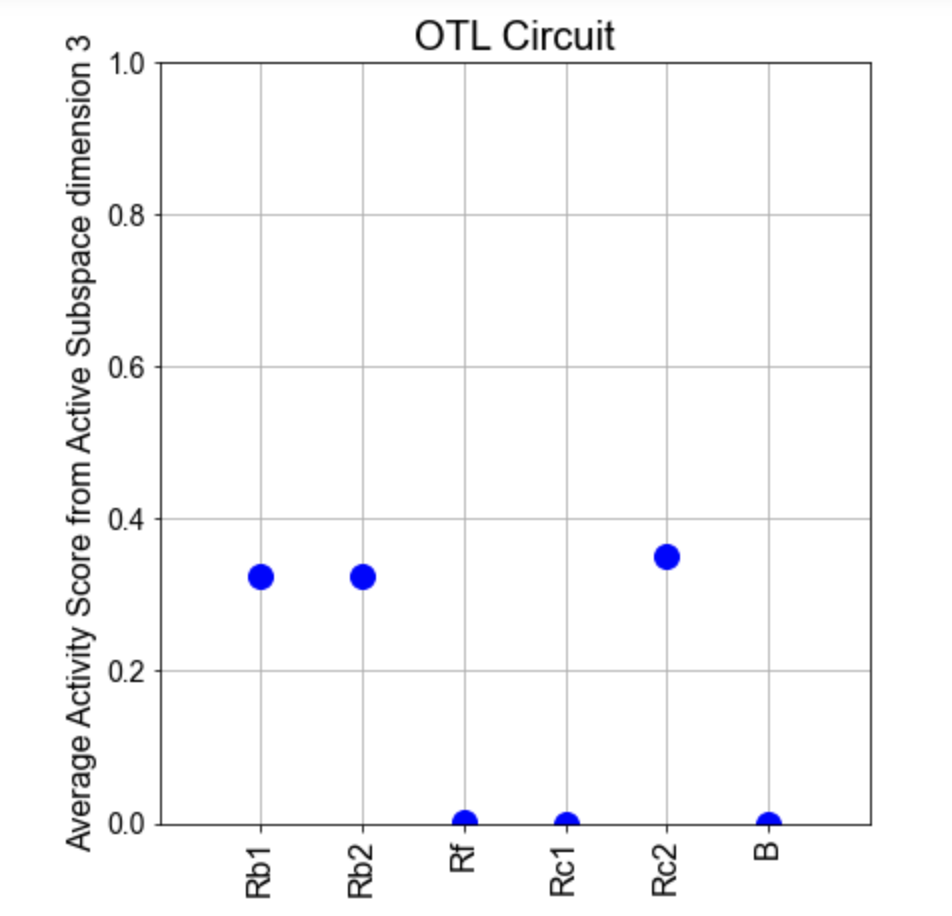
\includegraphics[height=1.25in,width=1.5in]{images/OTLEC2.png}
    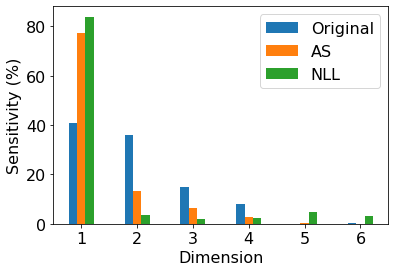
\includegraphics[height=1.25in,width=1.5in]{images/circuit sens.png}
    \captionsetup{justification=centering}
    \caption{Activity score and sensitivity comparison}
\end{subfigure}
\end{figure}
\end{frame}



\section{Conclusion}
\begin{frame}{Outcomes}
\begin{itemize}\itemsep20pt
    \item Understood the theoretical development of the AS and NLL methods for dimension reduction
    
    \item Learned to visualize the transformations provided by these methods, evaluate their performance, and determine the benefits and drawbacks of each method in various situations
    
    \item Used these methods for real-world applications in engineering
\end{itemize}
\end{frame}
\begin{frame}{Future Directions}
\begin{itemize}\itemsep20pt


    %\item In both the AS and NLL methods, we had to manually edit and choose certain code parameters, such as the method for gradient calculation in AS, and the learning rate, epochs, and time step in NLL. We used trial and error until we found a setup that modelled each function best. Ideally, a code could be written that does that work for you, and ensures that no better setups exist.
    
    \item Writing code to automate the process of finding optimal hyperparameters
    \begin{itemize}
        \item Could use sensitivity measures to evaluate the performance of the transformation created by certain hyperparameters
    \end{itemize}
    
    \item Further reducing computational costs by more efficiently approximating gradients and Jacobians
    
    \item Applying AS and NLL methods to vector-valued functions
    
    \item Using AS and NLL response surfaces for optimizing a function or estimating its average value
    
\end{itemize}
\end{frame}



\begin{frame}[allowframebreaks]{References}
\begin{itemize}
    \item \fullcite{constantine14}
    \item \fullcite{constantine15}
    \item \fullcite{NeurIPS19}
    \item \fullcite{athena}
    \item \fullcite{activesubspaces}
    \item \fullcite{wingfunction}
    \item \fullcite{pistonfunction}
    \item \fullcite{circuitfunction}
    \item \fullcite{ebola}
\end{itemize}
\end{frame}


\end{document}



